\section{Introduction}

As primitive objects in the Solar System, comets have the same physical and chemical properties as the planetary systems in the early Solar System, which can reveal information about the early Solar System. Research on comets can let us further understand the mechanism of planet formation and even solve some basic questions such as the origin of water on Earth. Unlike Short-peroid comets ($\mathrm{P}<\qty{200}{yr}$), most Long-period comets ($\mathrm{P}>\qty{200}{yr}$) originate from the Oort Cloud and are entering the inner Solar System for the first time. Long-period comets tend to exhibit stronger activity characteristics than Short-peroid comets do and appear brighter visually \ul{at the same heliocentric distance} due to the more volatile components they contain, comparing with the conventional water ice. 

Long-period comets also exhibit activity at large heliocentric distances more than {\qty{5}{\astronomicalunit}}. At this time, the activity is not caused by the sublimation effect of water ice. The current explanation about distant activity of comets mainly includes: the phase transition between amorphous and crystalline water ice \citep{prialnik_crystallization_1992, capria_c1995_2002}, the annealing of amorphous water ice \citep{meech_activity_2009}, and the sublimation of more volatile components such as \ce{CO2}~\citep{ootsubo_akari_2012} and/or \ce{CO}~\citep{jewitt_distant_2019}. 
% For comets that are active at a heliocentric distance of more than {\SI{4}{\astronomicalunit}} and whose nucleus surface temperature is lower than the \ce{H2O} sublimation temperature, their activity may be caused by the sublimation of more volatile \ce{CO2}~\citep{ootsubo_akari_2012} or \ce{CO}~\citep{jewitt_distant_2019}. In addition, \citet{ivanova_observations_2011} show that the upper layer of the comet nucleus should continue to peel off in order to conform to the observation results of long-term high activity of comets. 

Two Long-period comets C/2019 L3 and C/2020 P3 are selected for this study. They are all nearly isotropic, both of them having orbital semi-major axis more than {\SI{10000}{\astronomicalunit}}. C/2019 L3 and C/2020 P3 reach their perihelion on \DTMdate{2022-1-9} and \DTMdate{2021-4-21}\ul{, respectively}. Fig.~\ref{fig:orbit} shows the planar orbit graph of \st{them} \ul{two comets} in the Solar System. Table~\ref{tab:orb_elem} is the summary on orbital elements of these two comets. 

In this paper, we present broadband CCD photometry results of \st{the two comets metioned above} \ul{comets C/2019 L3 and C/2020 P3}. The circumstance of observations and data reduction process are presented in Section \ref{sec:obs_data}. Section \ref{sec:res} describes the photometry results, including morphology, surface brightness, $Af\rho$ and coma colors. Finally, discussion and conclusions are presented in Section \ref{sec:dis} and Section \ref {sec:con}. 

% orbital graph
\begin{figure}
    \centering
    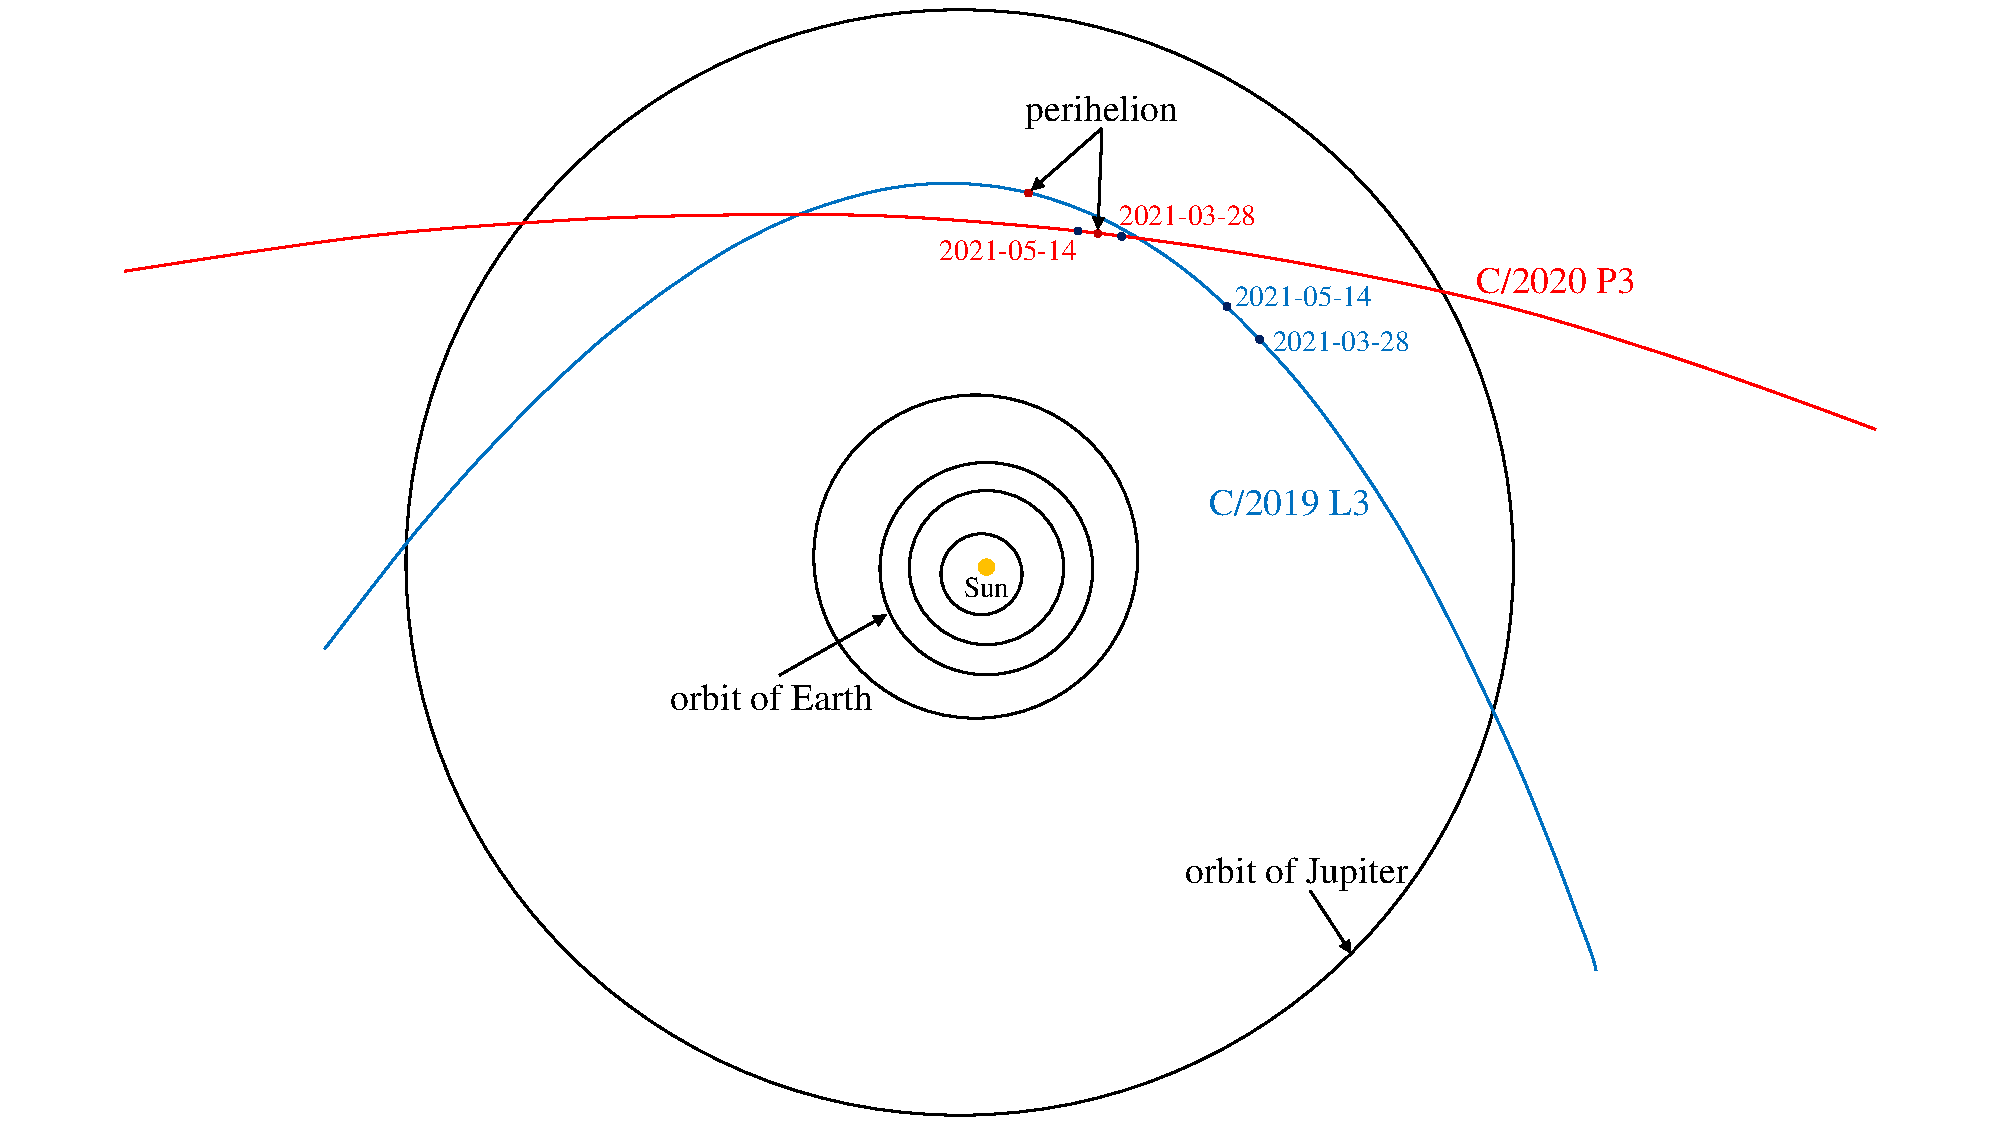
\includegraphics[width=1.0\columnwidth]{orbit.pdf}
    \caption{Orbit of comets C/2019 L3 and C/2020 P3 in the Solar System. The blue curve is the orbit of C/2019 L3 and the red curve is the orbit of C/2020 P3. Closed curves in black are the orbits of planets in the Solar System. Note that both of these comets have large orbital inclination not shown in this planar graph. The start and end dates of observations as well as the corresponding position of two objects on these dates are marked in this graph. }
    \label{fig:orbit}
\end{figure}

% orbital elements
\begin{table}
    \centering
    \caption{Orbital elements of comets C/2019 L3 and C/2020 P3 (Epoch: \DTMdate{2022-7-19}). }\label{tab:orb_elem}
    \begin{threeparttable}
        \resizebox{\linewidth}{!}{
        \begin{tabular}{ccccccccc}
            \toprule
            Comet & e\tnote{1} & q\tnote{2} & i\tnote{3} & $\Omega$\tnote{4} & $\omega$\tnote{5} & L\tnote{6} & B\tnote{7} & T\tnote{8} \\
            \midrule
            C/2019 L3       & \num{1.0017730}  & \num{3.5544290}  & \num{48.35710}  & \num{290.78850}  & \num{171.60970}  & \num{285.19094}  & \num{6.26014}   & \num{2459589.11650}  \\
            C/2020 P3       & \num{1.0003270}  & \num{6.8123330}  & \num{61.88790}  & \num{19.46850}   & \num{82.25590}   & \num{93.37021}   & \num{60.92485}  & \num{2459325.45200} \\
            \bottomrule
        \end{tabular}
        }
% 在正文介绍classification的部分
        \begin{tablenotes}
            \item[1] eccentricity 
            \item[2] perihelion distance
            \item[3] inclination
            \item[4] Longitude of ascending node
            \item[5] Argument of perihelion
            \item[6] Longitude of perihelion
            \item[7] Latitude of perihelion
            \item[8] Time of perihelion passage
        \end{tablenotes}
    \end{threeparttable}
\end{table}
